\documentclass{article}

\usepackage{multicol}
\usepackage{amsmath}
\usepackage{tikz}

\begin{document}


\hrulefill
\begin{multicols}{2}

    Obtain:

    \[
        \int{e^{x}\cos(x)}
    \]

    \columnbreak

    \begin{flushright}
        Answer: \[\frac{e^{x}}{2} \sin{\left (x \right )} + \frac{e^{x}}{2} \cos{\left (x \right )}\]
    \end{flushright}

\end{multicols}

\hrulefill
\begin{multicols}{2}

    Obtain:

    \[
        \lim_{x\to 1}\frac{x ^ 4 - 1}{x ^ 2 - 1}
    \]

    \columnbreak

    \begin{flushright}
        Answer: \[ 2 \]
    \end{flushright}

\end{multicols}


\hrulefill
\begin{multicols}{2}

    What is the long run stationary distribution of the following discrete time
    Markov chain:

    \begin{center}
        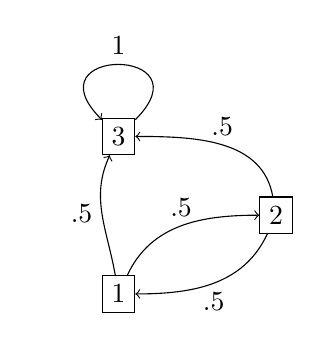
\begin{tikzpicture}
            \node (A) at (0, 0) [draw] {1};
            \node (B) at (2, 1) [draw] {2};
            \node (C) at (0, 2) [draw] {3};

            \draw [->] (A) to [out=65, in=180] node [above] {.5} (B);
            \draw [<-] (A) to [out=0, in=-115] node [below] {.5} (B);

            \draw [->] (A) to [out=100, in=-115] node [left] {.5} (C);
            \draw [->] (B) to [out=100, in=0] node [above] {.5} (C);

            \draw [->] (C) to [out=45, in=135, looseness=8] node [above] {1} (C);
        \end{tikzpicture}
    \end{center}

    \columnbreak

    Answer: \[ (0, 0, 1) \]

\end{multicols}



\hrulefill
\begin{multicols}{2}

    Minimize: \(4x + 12 y\)

    subject to:

    \begin{align*}
        x & \geq 0\\
        y & \geq 0\\
        5 x - y &\geq 2\\
        x + 2y &\leq 1
    \end{align*}
    

    \columnbreak

    Answer: \[ (x, y) = \left(\frac{5}{11}, \frac{3}{11}\right) \]

\end{multicols}

\hrulefill
\begin{multicols}{2}

    Obtain the mixed Nash equilibria for the following game:

    \[
        \begin{pmatrix}
            5, 6 & 1, 0\\
            0, 1 & 6, 5\\
        \end{pmatrix}
    \]

    \columnbreak

    Answer: \[ \left(\left(\frac{2}{5}, \frac{3}{5}\right), \left(\frac{1}{2}, \frac{1}{2}\right)\right) \]

\end{multicols}
\end{document}
